% Options for packages loaded elsewhere
\PassOptionsToPackage{unicode}{hyperref}
\PassOptionsToPackage{hyphens}{url}
\PassOptionsToPackage{dvipsnames,svgnames,x11names}{xcolor}
%
\documentclass[
  letterpaper,
  DIV=11,
  numbers=noendperiod,
  oneside]{scrreprt}

\usepackage{amsmath,amssymb}
\usepackage{iftex}
\ifPDFTeX
  \usepackage[T1]{fontenc}
  \usepackage[utf8]{inputenc}
  \usepackage{textcomp} % provide euro and other symbols
\else % if luatex or xetex
  \usepackage{unicode-math}
  \defaultfontfeatures{Scale=MatchLowercase}
  \defaultfontfeatures[\rmfamily]{Ligatures=TeX,Scale=1}
\fi
\usepackage{lmodern}
\ifPDFTeX\else  
    % xetex/luatex font selection
\fi
% Use upquote if available, for straight quotes in verbatim environments
\IfFileExists{upquote.sty}{\usepackage{upquote}}{}
\IfFileExists{microtype.sty}{% use microtype if available
  \usepackage[]{microtype}
  \UseMicrotypeSet[protrusion]{basicmath} % disable protrusion for tt fonts
}{}
\makeatletter
\@ifundefined{KOMAClassName}{% if non-KOMA class
  \IfFileExists{parskip.sty}{%
    \usepackage{parskip}
  }{% else
    \setlength{\parindent}{0pt}
    \setlength{\parskip}{6pt plus 2pt minus 1pt}}
}{% if KOMA class
  \KOMAoptions{parskip=half}}
\makeatother
\usepackage{xcolor}
\usepackage[left=1in,marginparwidth=2.0666666666667in,textwidth=4.1333333333333in,marginparsep=0.3in]{geometry}
\setlength{\emergencystretch}{3em} % prevent overfull lines
\setcounter{secnumdepth}{5}
% Make \paragraph and \subparagraph free-standing
\makeatletter
\ifx\paragraph\undefined\else
  \let\oldparagraph\paragraph
  \renewcommand{\paragraph}{
    \@ifstar
      \xxxParagraphStar
      \xxxParagraphNoStar
  }
  \newcommand{\xxxParagraphStar}[1]{\oldparagraph*{#1}\mbox{}}
  \newcommand{\xxxParagraphNoStar}[1]{\oldparagraph{#1}\mbox{}}
\fi
\ifx\subparagraph\undefined\else
  \let\oldsubparagraph\subparagraph
  \renewcommand{\subparagraph}{
    \@ifstar
      \xxxSubParagraphStar
      \xxxSubParagraphNoStar
  }
  \newcommand{\xxxSubParagraphStar}[1]{\oldsubparagraph*{#1}\mbox{}}
  \newcommand{\xxxSubParagraphNoStar}[1]{\oldsubparagraph{#1}\mbox{}}
\fi
\makeatother

\usepackage{color}
\usepackage{fancyvrb}
\newcommand{\VerbBar}{|}
\newcommand{\VERB}{\Verb[commandchars=\\\{\}]}
\DefineVerbatimEnvironment{Highlighting}{Verbatim}{commandchars=\\\{\}}
% Add ',fontsize=\small' for more characters per line
\usepackage{framed}
\definecolor{shadecolor}{RGB}{241,243,245}
\newenvironment{Shaded}{\begin{snugshade}}{\end{snugshade}}
\newcommand{\AlertTok}[1]{\textcolor[rgb]{0.68,0.00,0.00}{#1}}
\newcommand{\AnnotationTok}[1]{\textcolor[rgb]{0.37,0.37,0.37}{#1}}
\newcommand{\AttributeTok}[1]{\textcolor[rgb]{0.40,0.45,0.13}{#1}}
\newcommand{\BaseNTok}[1]{\textcolor[rgb]{0.68,0.00,0.00}{#1}}
\newcommand{\BuiltInTok}[1]{\textcolor[rgb]{0.00,0.23,0.31}{#1}}
\newcommand{\CharTok}[1]{\textcolor[rgb]{0.13,0.47,0.30}{#1}}
\newcommand{\CommentTok}[1]{\textcolor[rgb]{0.37,0.37,0.37}{#1}}
\newcommand{\CommentVarTok}[1]{\textcolor[rgb]{0.37,0.37,0.37}{\textit{#1}}}
\newcommand{\ConstantTok}[1]{\textcolor[rgb]{0.56,0.35,0.01}{#1}}
\newcommand{\ControlFlowTok}[1]{\textcolor[rgb]{0.00,0.23,0.31}{\textbf{#1}}}
\newcommand{\DataTypeTok}[1]{\textcolor[rgb]{0.68,0.00,0.00}{#1}}
\newcommand{\DecValTok}[1]{\textcolor[rgb]{0.68,0.00,0.00}{#1}}
\newcommand{\DocumentationTok}[1]{\textcolor[rgb]{0.37,0.37,0.37}{\textit{#1}}}
\newcommand{\ErrorTok}[1]{\textcolor[rgb]{0.68,0.00,0.00}{#1}}
\newcommand{\ExtensionTok}[1]{\textcolor[rgb]{0.00,0.23,0.31}{#1}}
\newcommand{\FloatTok}[1]{\textcolor[rgb]{0.68,0.00,0.00}{#1}}
\newcommand{\FunctionTok}[1]{\textcolor[rgb]{0.28,0.35,0.67}{#1}}
\newcommand{\ImportTok}[1]{\textcolor[rgb]{0.00,0.46,0.62}{#1}}
\newcommand{\InformationTok}[1]{\textcolor[rgb]{0.37,0.37,0.37}{#1}}
\newcommand{\KeywordTok}[1]{\textcolor[rgb]{0.00,0.23,0.31}{\textbf{#1}}}
\newcommand{\NormalTok}[1]{\textcolor[rgb]{0.00,0.23,0.31}{#1}}
\newcommand{\OperatorTok}[1]{\textcolor[rgb]{0.37,0.37,0.37}{#1}}
\newcommand{\OtherTok}[1]{\textcolor[rgb]{0.00,0.23,0.31}{#1}}
\newcommand{\PreprocessorTok}[1]{\textcolor[rgb]{0.68,0.00,0.00}{#1}}
\newcommand{\RegionMarkerTok}[1]{\textcolor[rgb]{0.00,0.23,0.31}{#1}}
\newcommand{\SpecialCharTok}[1]{\textcolor[rgb]{0.37,0.37,0.37}{#1}}
\newcommand{\SpecialStringTok}[1]{\textcolor[rgb]{0.13,0.47,0.30}{#1}}
\newcommand{\StringTok}[1]{\textcolor[rgb]{0.13,0.47,0.30}{#1}}
\newcommand{\VariableTok}[1]{\textcolor[rgb]{0.07,0.07,0.07}{#1}}
\newcommand{\VerbatimStringTok}[1]{\textcolor[rgb]{0.13,0.47,0.30}{#1}}
\newcommand{\WarningTok}[1]{\textcolor[rgb]{0.37,0.37,0.37}{\textit{#1}}}

\providecommand{\tightlist}{%
  \setlength{\itemsep}{0pt}\setlength{\parskip}{0pt}}\usepackage{longtable,booktabs,array}
\usepackage{calc} % for calculating minipage widths
% Correct order of tables after \paragraph or \subparagraph
\usepackage{etoolbox}
\makeatletter
\patchcmd\longtable{\par}{\if@noskipsec\mbox{}\fi\par}{}{}
\makeatother
% Allow footnotes in longtable head/foot
\IfFileExists{footnotehyper.sty}{\usepackage{footnotehyper}}{\usepackage{footnote}}
\makesavenoteenv{longtable}
\usepackage{graphicx}
\makeatletter
\newsavebox\pandoc@box
\newcommand*\pandocbounded[1]{% scales image to fit in text height/width
  \sbox\pandoc@box{#1}%
  \Gscale@div\@tempa{\textheight}{\dimexpr\ht\pandoc@box+\dp\pandoc@box\relax}%
  \Gscale@div\@tempb{\linewidth}{\wd\pandoc@box}%
  \ifdim\@tempb\p@<\@tempa\p@\let\@tempa\@tempb\fi% select the smaller of both
  \ifdim\@tempa\p@<\p@\scalebox{\@tempa}{\usebox\pandoc@box}%
  \else\usebox{\pandoc@box}%
  \fi%
}
% Set default figure placement to htbp
\def\fps@figure{htbp}
\makeatother

\KOMAoption{captions}{tableheading}
\makeatletter
\@ifpackageloaded{tcolorbox}{}{\usepackage[skins,breakable]{tcolorbox}}
\@ifpackageloaded{fontawesome5}{}{\usepackage{fontawesome5}}
\definecolor{quarto-callout-color}{HTML}{909090}
\definecolor{quarto-callout-note-color}{HTML}{0758E5}
\definecolor{quarto-callout-important-color}{HTML}{CC1914}
\definecolor{quarto-callout-warning-color}{HTML}{EB9113}
\definecolor{quarto-callout-tip-color}{HTML}{00A047}
\definecolor{quarto-callout-caution-color}{HTML}{FC5300}
\definecolor{quarto-callout-color-frame}{HTML}{acacac}
\definecolor{quarto-callout-note-color-frame}{HTML}{4582ec}
\definecolor{quarto-callout-important-color-frame}{HTML}{d9534f}
\definecolor{quarto-callout-warning-color-frame}{HTML}{f0ad4e}
\definecolor{quarto-callout-tip-color-frame}{HTML}{02b875}
\definecolor{quarto-callout-caution-color-frame}{HTML}{fd7e14}
\makeatother
\makeatletter
\@ifpackageloaded{bookmark}{}{\usepackage{bookmark}}
\makeatother
\makeatletter
\@ifpackageloaded{caption}{}{\usepackage{caption}}
\AtBeginDocument{%
\ifdefined\contentsname
  \renewcommand*\contentsname{Table of contents}
\else
  \newcommand\contentsname{Table of contents}
\fi
\ifdefined\listfigurename
  \renewcommand*\listfigurename{List of Figures}
\else
  \newcommand\listfigurename{List of Figures}
\fi
\ifdefined\listtablename
  \renewcommand*\listtablename{List of Tables}
\else
  \newcommand\listtablename{List of Tables}
\fi
\ifdefined\figurename
  \renewcommand*\figurename{Figure}
\else
  \newcommand\figurename{Figure}
\fi
\ifdefined\tablename
  \renewcommand*\tablename{Table}
\else
  \newcommand\tablename{Table}
\fi
}
\@ifpackageloaded{float}{}{\usepackage{float}}
\floatstyle{ruled}
\@ifundefined{c@chapter}{\newfloat{codelisting}{h}{lop}}{\newfloat{codelisting}{h}{lop}[chapter]}
\floatname{codelisting}{Listing}
\newcommand*\listoflistings{\listof{codelisting}{List of Listings}}
\makeatother
\makeatletter
\makeatother
\makeatletter
\@ifpackageloaded{caption}{}{\usepackage{caption}}
\@ifpackageloaded{subcaption}{}{\usepackage{subcaption}}
\makeatother
\makeatletter
\@ifpackageloaded{sidenotes}{}{\usepackage{sidenotes}}
\@ifpackageloaded{marginnote}{}{\usepackage{marginnote}}
\makeatother

\usepackage{bookmark}

\IfFileExists{xurl.sty}{\usepackage{xurl}}{} % add URL line breaks if available
\urlstyle{same} % disable monospaced font for URLs
\hypersetup{
  pdftitle={Rust for R Developers},
  pdfauthor={Josiah Parry},
  colorlinks=true,
  linkcolor={blue},
  filecolor={Maroon},
  citecolor={Blue},
  urlcolor={Blue},
  pdfcreator={LaTeX via pandoc}}


\title{Rust for R Developers}
\usepackage{etoolbox}
\makeatletter
\providecommand{\subtitle}[1]{% add subtitle to \maketitle
  \apptocmd{\@title}{\par {\large #1 \par}}{}{}
}
\makeatother
\subtitle{Cascadia R Conference, 2025}
\author{Josiah Parry}
\date{2025-06-20}

\begin{document}
\maketitle

\renewcommand*\contentsname{Table of contents}
{
\hypersetup{linkcolor=}
\setcounter{tocdepth}{2}
\tableofcontents
}

\bookmarksetup{startatroot}

\chapter{Get set up}\label{get-set-up}

\section{Setting up}\label{setting-up}

Before we can start, we need to get our house in order. We need to
install:

\begin{itemize}
\tightlist
\item[$\square$]
  Positron
\item[$\square$]
  Rust
\item[$\square$]
  \href{https://marketplace.visualstudio.com/items?itemName=rust-lang.rust-analyzer}{Rust
  analyzer VS Code extension}
\item[$\square$]
  \href{https://marketplace.visualstudio.com/items?itemName=tamasfe.even-better-toml}{Even
  Better TOML VS Code extension}
\end{itemize}

\section{Install Positron}\label{install-positron}

Download the appropriate Positron installer from the
\href{https://positron.posit.co/download.html}{downloads page}.

Open the extensions pane (or press \texttt{shift\ +\ cmd\ +\ x}).

\begin{itemize}
\tightlist
\item
  search for \texttt{rust\ analyzer} and install
\item
  search for \texttt{even\ better\ toml} and install
\end{itemize}

\section{Install rust}\label{install-rust}

To install Rust, please use \href{https://rustup.rs/}{rustup}. If you
use a system installation via brew, apt, dnf, etc you will likely run
into issues. I will be able to help debug these.

For installing Rust on Mac / Unix / Linux please run:

\begin{Shaded}
\begin{Highlighting}[]
\NormalTok{curl {-}{-}proto \textquotesingle{}=https\textquotesingle{} {-}{-}tlsv1.2 {-}sSf https://sh.rustup.rs | sh}
\end{Highlighting}
\end{Shaded}

\subsection{Windows}\label{windows}

If using Windows download the appropriate installer. Then, once your
installation is complete, from your command prompt run:

\begin{Shaded}
\begin{Highlighting}[]
\NormalTok{rustup target add x86\_64{-}pc{-}windows{-}gnu}
\end{Highlighting}
\end{Shaded}

This is a compilation target that is required for building extendr
packages on Windows.

\part{Intro to Rust for R Developers}

\chapter{Overview}\label{overview}

\section{Timeline}\label{timeline}

We've got 3 hours to cover a lot of ground!

\begin{itemize}
\tightlist
\item
  What is rust
\item
  Hello, World!
\item
  Primitive types, logical operators, and control flow
\item
  Creating Functions
\item
  Arrays \& vectors
\item
  For loops
\item
  Mutability
\item
  Iterators
\item
  References and Slices
\item
  Structs
\end{itemize}

\begin{longtable}[]{@{}ll@{}}
\toprule\noalign{}
Start & Description \\
\midrule\noalign{}
\endhead
\bottomrule\noalign{}
\endlastfoot
\end{longtable}

\chapter{Why Rust?}\label{why-rust}

\begin{tcolorbox}[enhanced jigsaw, titlerule=0mm, coltitle=black, opacitybacktitle=0.6, bottomrule=.15mm, bottomtitle=1mm, colframe=quarto-callout-tip-color-frame, toprule=.15mm, opacityback=0, rightrule=.15mm, leftrule=.75mm, breakable, left=2mm, colback=white, colbacktitle=quarto-callout-tip-color!10!white, toptitle=1mm, title=\textcolor{quarto-callout-tip-color}{\faLightbulb}\hspace{0.5em}{Objective}, arc=.35mm]

Provide motivation for \emph{why} learning Rust is a use of our time.
Discuss \emph{what} Rust is and how it is unique compared to other
compiled langauges.

🧠 Think of Rust as ``C for people who like error messages that actually
help.''

\end{tcolorbox}

\section{Reasoning}\label{reasoning}

Rust is a programming language that's fast, safe, and surprisingly
friendly to use. Unlike R, which runs code line by line, Rust turns your
code into a standalone program that runs directly on your computer. This
makes it much faster and more efficient, similar to languages like C or
C++. But where those languages can be hard to use and easy to break,
Rust was built to be safer and more helpful.

Rust is especially good at preventing bugs related to memory and
parallel code --- the kind that can be really hard to track down in
other languages. And it comes with tools and error messages that make
writing and fixing code feel more approachable, even if you're new to
systems programming. Many R users find Rust refreshing: it's strict, but
in a way that teaches you better habits.

\section{TL;DR}\label{tldr}

\begin{itemize}
\tightlist
\item
  R is interpreted. Code runs line by line.
\item
  R (and Python) are built on C.
\item
  C is compiled --- it builds a binary that runs directly on your
  machine.
\item
  Rust is also compiled, like C, C++, Go, Java, and Fortran.
\item
  These languages are ``close to the metal'' --- fast, efficient, and
  powerful.
\item
  Rust matches C++ in speed, but with some key advantages:

  \begin{itemize}
  \tightlist
  \item
    \textbf{Memory safety} without a garbage collector (unlike Go),
    thanks to the borrow checker.
  \item
    \textbf{Fearless concurrency} --- Rust makes parallelism safer and
    easier.
  \item
    A great developer experience:

    \begin{itemize}
    \tightlist
    \item
      Helpful, friendly compiler errors (Tidyverse-level DX).
    \item
      Modern tooling (cargo, rust-analyzer, etc.).
    \end{itemize}
  \end{itemize}
\item
  Rust is easy to get started with and rewards best practices.

  \begin{itemize}
  \tightlist
  \item
    We won't go deep into memory safety or concurrency today
  \end{itemize}
\end{itemize}

\chapter{Hello, World!}\label{hello-world}

\begin{tcolorbox}[enhanced jigsaw, titlerule=0mm, coltitle=black, opacitybacktitle=0.6, bottomrule=.15mm, bottomtitle=1mm, colframe=quarto-callout-tip-color-frame, toprule=.15mm, opacityback=0, rightrule=.15mm, leftrule=.75mm, breakable, left=2mm, colback=white, colbacktitle=quarto-callout-tip-color!10!white, toptitle=1mm, title=\textcolor{quarto-callout-tip-color}{\faLightbulb}\hspace{0.5em}{Objective}, arc=.35mm]

\begin{itemize}
\tightlist
\item
  Create a rust crate
\item
  Understand the structure of a rust crate
\item
  Use \texttt{cargo\ run} to run a binary
\item
  Use the \texttt{println!()} macro
\end{itemize}

\end{tcolorbox}

Rust uses a tool called \texttt{cargo} for building, checking, and
managing dependencies.

To create a new Rust crate, use \texttt{cargo\ new\ name-of-crate}.

\section{Crate anatomy}\label{crate-anatomy}

Two types of crates: binary, library.

\marginnote{\begin{footnotesize}

This first workshop we will work only with a binary crate. We will
create a library in the second half of the day.

\end{footnotesize}}

Binary crates are standalone applications like command line tools, or
things that run once---simiar to a script that you run with
\texttt{Rscript\ main.R}

\section{Crate anatomy}\label{crate-anatomy-1}

A new crate looks like this:

\begin{verbatim}
intro-to-rust/
├── Cargo.toml      # Metadata & dependencies (like DESCRIPTION)
├── Cargo.lock      # Dependency versions (like renv.lock)
└── src/
    └── main.rs     # Entry point — like main.R
\end{verbatim}

\section{\texorpdfstring{\texttt{main.rs}}{main.rs}}\label{main.rs}

When you create a new rust binary the file \texttt{src/main.rs} is
prepopulated with:

\begin{tcolorbox}[enhanced jigsaw, titlerule=0mm, coltitle=black, opacitybacktitle=0.6, bottomrule=.15mm, bottomtitle=1mm, colframe=quarto-callout-tip-color-frame, toprule=.15mm, opacityback=0, rightrule=.15mm, leftrule=.75mm, breakable, left=2mm, colback=white, colbacktitle=quarto-callout-tip-color!10!white, toptitle=1mm, title=\textcolor{quarto-callout-tip-color}{\faLightbulb}\hspace{0.5em}{Tip}, arc=.35mm]

\texttt{src/main.rs} defines what is executed when your \emph{binary} is
run.

\end{tcolorbox}

\begin{Shaded}
\begin{Highlighting}[]
\KeywordTok{fn}\NormalTok{ main() }\OperatorTok{\{}
    \PreprocessorTok{println!}\NormalTok{(}\StringTok{"Hello, world!"}\NormalTok{)}\OperatorTok{;}
\OperatorTok{\}}
\end{Highlighting}
\end{Shaded}

There are a few things going on in here:

\begin{itemize}
\tightlist
\item
  Functions are declared using the \texttt{fn} keyword
\item
  The \texttt{main()} function is the entrypoint of the program (and
  required)
\item
  Blocks of code are delimted using curly braces (like R \& C)
\item
  Statements end with \texttt{;}
\item
  \texttt{println!()} is a macro (notice the \texttt{!}) which is used
  to print to \texttt{stdout}
\end{itemize}

\marginnote{\begin{footnotesize}

When a program writes to the console it does so through file connections
called standard output (\texttt{stdout}) and standard error
(\texttt{stderr}).

When we print a message with \texttt{print()} or \texttt{message()} in
R, we print to stdout. When we make a warning or error using
\texttt{stop()} or \texttt{warning()} in R, that is writing to
\texttt{stderr}.

\end{footnotesize}}

\section{\texorpdfstring{\texttt{println!()}}{println!()}}\label{println}

\begin{itemize}
\tightlist
\item
  Macros have a \texttt{!}, like \texttt{println!()}.
\item
  Think of it like \texttt{print()} in R, but explicit.
\item
  It supports format strings:
\end{itemize}

\begin{Shaded}
\begin{Highlighting}[]
\KeywordTok{let}\NormalTok{ name }\OperatorTok{=} \StringTok{"Josiah"}\OperatorTok{;}
\PreprocessorTok{println!}\NormalTok{(}\StringTok{"Hello, \{\}!"}\OperatorTok{,}\NormalTok{ name)}\OperatorTok{;}  \CommentTok{// {-}\textgreater{} Hello, Josiah!}
\end{Highlighting}
\end{Shaded}

\section{Exercise}\label{exercise}

\begin{itemize}
\tightlist
\item
  In your terminal, create a new rust crate called
  \texttt{intro-to-rust}
\item
  Open the new rust crate in Positron
\item
  Run the hello world program
\item
  Create variable called \texttt{name} with your name
\item
  Print \texttt{Hello,\ \{name\}!} using \texttt{println!()}
\end{itemize}

\subsection{Solution}\label{solution}

View solution

In \texttt{src/main.rs}

\begin{Shaded}
\begin{Highlighting}[]
\KeywordTok{fn}\NormalTok{ main() }\OperatorTok{\{}
    \KeywordTok{let}\NormalTok{ name }\OperatorTok{=} \StringTok{"Josiah"}\OperatorTok{;}
    \PreprocessorTok{println!}\NormalTok{(}\StringTok{"Hello, \{name\}!"}\NormalTok{)}\OperatorTok{;}
\OperatorTok{\}}
\end{Highlighting}
\end{Shaded}

To run it navigate to your terminal and then run \texttt{cargo\ run}.

\chapter{Control Flow}\label{control-flow}

\begin{tcolorbox}[enhanced jigsaw, titlerule=0mm, coltitle=black, opacitybacktitle=0.6, bottomrule=.15mm, bottomtitle=1mm, colframe=quarto-callout-tip-color-frame, toprule=.15mm, opacityback=0, rightrule=.15mm, leftrule=.75mm, breakable, left=2mm, colback=white, colbacktitle=quarto-callout-tip-color!10!white, toptitle=1mm, title=\textcolor{quarto-callout-tip-color}{\faLightbulb}\hspace{0.5em}{Objective}, arc=.35mm]

Understand control flow and numeric operators in Rust. You will create
the FizzBuzz program using Rust!

\end{tcolorbox}

\section{Numeric operators}\label{numeric-operators}

\begin{itemize}
\tightlist
\item
  \texttt{+} addition
\item
  \texttt{-} subtraction
\item
  \texttt{/} division
\item
  \texttt{\^{}} exponentiation
\item
  \texttt{\%} remainder
\end{itemize}

\section{Logical Operators:}\label{logical-operators}

Logical operators are quite similar to R. The key differe

\begin{itemize}
\tightlist
\item
  \texttt{==} check equality
\item
  \texttt{!=} check inequality
\item
  \texttt{!} negate a logical value
\item
  \texttt{\&\&} logical AND comparison
\item
  \texttt{\textbar{}\textbar{}} logical OR comparison
\end{itemize}

\section{Control flow}\label{control-flow-1}

Rust uses \texttt{if}, \texttt{else}, and \texttt{else\ if} statements
just like R. Where each branch is delimted by curly braces.

\begin{tcolorbox}[enhanced jigsaw, titlerule=0mm, coltitle=black, opacitybacktitle=0.6, bottomrule=.15mm, bottomtitle=1mm, colframe=quarto-callout-warning-color-frame, toprule=.15mm, opacityback=0, rightrule=.15mm, leftrule=.75mm, breakable, left=2mm, colback=white, colbacktitle=quarto-callout-warning-color!10!white, toptitle=1mm, title=\textcolor{quarto-callout-warning-color}{\faExclamationTriangle}\hspace{0.5em}{Warning}, arc=.35mm]

Each branch of the \texttt{if} statement must return the same type. For
this portion of the workshop, be sure to \textbf{terminate} each
statement inside of the \texttt{if} statement so that nothing is
returned.

\end{tcolorbox}

\begin{Shaded}
\begin{Highlighting}[]
\ControlFlowTok{if}\NormalTok{ x }\OperatorTok{==}\NormalTok{ y }\OperatorTok{\{}
  \CommentTok{// do something}
\OperatorTok{\}} \ControlFlowTok{else} \OperatorTok{\{}
  \CommentTok{// do something else}
\OperatorTok{\}}
\end{Highlighting}
\end{Shaded}

The key difference is that the use of parentheses is not necessary for
the conditional statement.

\section{Exercise}\label{exercise-1}

This exercise you will create the famous FizzBuzz program.

For this, create a variable \texttt{i}. The rules are:

\begin{itemize}
\tightlist
\item
  when \texttt{i} is a multiple of \texttt{3}, print \texttt{Fizz}
\item
  when \texttt{i} is a multiple of \texttt{5}, print \texttt{Buzz}
\item
  when \texttt{i} is a multiple of \emph{both} \texttt{3} and
  \texttt{5}, print \texttt{FizzBuzz}
\end{itemize}

\subsection{Solution}\label{solution-1}

View solution

\begin{Shaded}
\begin{Highlighting}[]
\KeywordTok{fn}\NormalTok{ main() }\OperatorTok{\{}
    \CommentTok{// let i = 15; // FizzBuzz}
    \CommentTok{// let i = 3; // Fizz}
    \CommentTok{// let i = 5; // Buzz}
    \KeywordTok{let}\NormalTok{ i }\OperatorTok{=} \DecValTok{47}\OperatorTok{;} \CommentTok{// Nothing}
    \ControlFlowTok{if}\NormalTok{ (i }\OperatorTok{\%} \DecValTok{3} \OperatorTok{==} \DecValTok{0}\NormalTok{) }\OperatorTok{\&\&}\NormalTok{ (i }\OperatorTok{\%} \DecValTok{5} \OperatorTok{==} \DecValTok{0}\NormalTok{) }\OperatorTok{\{}
        \PreprocessorTok{println!}\NormalTok{(}\StringTok{"FizzBuzz"}\NormalTok{)}\OperatorTok{;}
    \OperatorTok{\}} \ControlFlowTok{else} \ControlFlowTok{if}\NormalTok{ i }\OperatorTok{\%} \DecValTok{3} \OperatorTok{==} \DecValTok{0} \OperatorTok{\{}
        \PreprocessorTok{println!}\NormalTok{(}\StringTok{"Fizz"}\NormalTok{)}\OperatorTok{;}
    \OperatorTok{\}} \ControlFlowTok{else} \ControlFlowTok{if}\NormalTok{ i }\OperatorTok{\%} \DecValTok{5} \OperatorTok{==} \DecValTok{0} \OperatorTok{\{}
        \PreprocessorTok{println!}\NormalTok{(}\StringTok{"Buzz"}\NormalTok{)}\OperatorTok{;}
    \OperatorTok{\}}
\OperatorTok{\}}
\end{Highlighting}
\end{Shaded}

\chapter{Arrays and Vectors}\label{arrays-and-vectors}

\begin{tcolorbox}[enhanced jigsaw, titlerule=0mm, coltitle=black, opacitybacktitle=0.6, bottomrule=.15mm, bottomtitle=1mm, colframe=quarto-callout-tip-color-frame, toprule=.15mm, opacityback=0, rightrule=.15mm, leftrule=.75mm, breakable, left=2mm, colback=white, colbacktitle=quarto-callout-tip-color!10!white, toptitle=1mm, title=\textcolor{quarto-callout-tip-color}{\faLightbulb}\hspace{0.5em}{Objective}, arc=.35mm]

\begin{itemize}
\tightlist
\item
  Create and store many values of the same type.
\item
  Understand the difference between arrays and vectors.
\end{itemize}

\end{tcolorbox}

\section{Arrays}\label{arrays}

Arrays in Rust are fixed in size and hold values of the same type. Since
the size is known ahead of time, it makes them fast but inflexible.

\begin{Shaded}
\begin{Highlighting}[]
\KeywordTok{fn}\NormalTok{ main() }\OperatorTok{\{}
    \KeywordTok{let}\NormalTok{ arr }\OperatorTok{=}\NormalTok{ [}\DecValTok{10}\OperatorTok{,} \DecValTok{20}\OperatorTok{,} \DecValTok{30}\OperatorTok{,} \DecValTok{40}\NormalTok{]}\OperatorTok{;}
    \PreprocessorTok{println!}\NormalTok{(}\StringTok{"Array: \{:?\}"}\OperatorTok{,}\NormalTok{ arr)}\OperatorTok{;}
\OperatorTok{\}}
\end{Highlighting}
\end{Shaded}

\begin{tcolorbox}[enhanced jigsaw, titlerule=0mm, coltitle=black, opacitybacktitle=0.6, bottomrule=.15mm, bottomtitle=1mm, colframe=quarto-callout-note-color-frame, toprule=.15mm, opacityback=0, rightrule=.15mm, leftrule=.75mm, breakable, left=2mm, colback=white, colbacktitle=quarto-callout-note-color!10!white, toptitle=1mm, title=\textcolor{quarto-callout-note-color}{\faInfo}\hspace{0.5em}{Note}, arc=.35mm]

The \texttt{\{:?\}} syntax is used for a
\href{https://doc.rust-lang.org/std/fmt/trait.Debug.html}{\textbf{Debug}}
representation of a variable. Using \texttt{\{\}} is used for
\href{https://doc.rust-lang.org/std/fmt/trait.Display.html}{\textbf{Displaying}}
data.

More often than not, using \texttt{\{:?\}} will be your best option.

\end{tcolorbox}

\begin{itemize}
\tightlist
\item
  Arrays use square brackets: \texttt{{[}1,\ 2,\ 3{]}}
\item
  Their size is known at compile time.
\item
  You can't add or remove elements.
\item
  Mostly used when performance is critical and size is known.
\end{itemize}

\section{Vectors}\label{vectors}

Vectors are like growable arrays. They live on the heap and are much
more common in everyday Rust code. We'll explore how to modify them
later, but for now, we can define them with values known at the start.

\begin{Shaded}
\begin{Highlighting}[]
\KeywordTok{fn}\NormalTok{ main() }\OperatorTok{\{}
    \KeywordTok{let}\NormalTok{ v }\OperatorTok{=} \PreprocessorTok{vec!}\NormalTok{[}\DecValTok{1}\OperatorTok{,} \DecValTok{2}\OperatorTok{,} \DecValTok{3}\OperatorTok{,} \DecValTok{4}\OperatorTok{,} \DecValTok{5}\NormalTok{]}\OperatorTok{;}
    \PreprocessorTok{println!}\NormalTok{(}\StringTok{"Vector: \{:?\}"}\OperatorTok{,}\NormalTok{ v)}\OperatorTok{;}
\OperatorTok{\}}
\end{Highlighting}
\end{Shaded}

\begin{itemize}
\tightlist
\item
  Create vectors using \texttt{vec!{[}{]}}
\item
  You don't need \texttt{mut} if you're not changing them.
\item
  Like arrays, all values must be the same type.
\end{itemize}

In R, most things are vectorized. In Rust, we often \textbf{iterate}
over collections to work with them.

\section{Exercise}\label{exercise-2}

\begin{itemize}
\tightlist
\item
  Create an array of 4 integers and print it.
\item
  Create a vector with 5 numbers and print it using \texttt{\{:?\}}.
\end{itemize}

\subsection{Solution}\label{solution-2}

View solution

\begin{Shaded}
\begin{Highlighting}[]
\KeywordTok{fn}\NormalTok{ main() }\OperatorTok{\{}
    \KeywordTok{let}\NormalTok{ arr }\OperatorTok{=}\NormalTok{ [}\DecValTok{1}\OperatorTok{,} \DecValTok{2}\OperatorTok{,} \DecValTok{3}\OperatorTok{,} \DecValTok{4}\NormalTok{]}\OperatorTok{;}
    \PreprocessorTok{println!}\NormalTok{(}\StringTok{"Array: \{:?\}"}\OperatorTok{,}\NormalTok{ arr)}\OperatorTok{;}

    \KeywordTok{let}\NormalTok{ v }\OperatorTok{=} \PreprocessorTok{vec!}\NormalTok{[}\DecValTok{10}\OperatorTok{,} \DecValTok{20}\OperatorTok{,} \DecValTok{30}\OperatorTok{,} \DecValTok{40}\OperatorTok{,} \DecValTok{50}\NormalTok{]}\OperatorTok{;}
    \PreprocessorTok{println!}\NormalTok{(}\StringTok{"Vector: \{:?\}"}\OperatorTok{,}\NormalTok{ v)}\OperatorTok{;}
\OperatorTok{\}}
\end{Highlighting}
\end{Shaded}

\begin{center}\rule{0.5\linewidth}{0.5pt}\end{center}

NOTES:

TODO:

add a bit on \texttt{.len()} and \texttt{.is\_empty()}

\chapter{For Loops}\label{for-loops}

\begin{tcolorbox}[enhanced jigsaw, titlerule=0mm, coltitle=black, opacitybacktitle=0.6, bottomrule=.15mm, bottomtitle=1mm, colframe=quarto-callout-tip-color-frame, toprule=.15mm, opacityback=0, rightrule=.15mm, leftrule=.75mm, breakable, left=2mm, colback=white, colbacktitle=quarto-callout-tip-color!10!white, toptitle=1mm, title=\textcolor{quarto-callout-tip-color}{\faLightbulb}\hspace{0.5em}{Objective}, arc=.35mm]

\begin{itemize}
\tightlist
\item
  Learn how to loop over a collection of values.
\item
  Apply logic to each value inside a loop.
\end{itemize}

\end{tcolorbox}

\section{\texorpdfstring{\texttt{for} loop
syntax}{for loop syntax}}\label{for-loop-syntax}

\begin{Shaded}
\begin{Highlighting}[]
\ControlFlowTok{for}\NormalTok{ value }\KeywordTok{in}\NormalTok{ collection }\OperatorTok{\{}
    \CommentTok{// do something with value}
\OperatorTok{\}}
\end{Highlighting}
\end{Shaded}

In Rust, \texttt{for} loops are the easiest way to go over each item in
a vector or array.

\begin{Shaded}
\begin{Highlighting}[]
\KeywordTok{fn}\NormalTok{ main() }\OperatorTok{\{}
    \KeywordTok{let}\NormalTok{ nums }\OperatorTok{=} \PreprocessorTok{vec!}\NormalTok{[}\DecValTok{1}\OperatorTok{,} \DecValTok{2}\OperatorTok{,} \DecValTok{3}\NormalTok{]}\OperatorTok{;}
    \ControlFlowTok{for}\NormalTok{ n }\KeywordTok{in}\NormalTok{ nums }\OperatorTok{\{}
        \PreprocessorTok{println!}\NormalTok{(}\StringTok{"n is: \{\}"}\OperatorTok{,}\NormalTok{ n)}\OperatorTok{;}
    \OperatorTok{\}}
\OperatorTok{\}}
\end{Highlighting}
\end{Shaded}

\section{Scope}\label{scope}

\begin{itemize}
\tightlist
\item
  Values \emph{outside} of the for loop are accessible inside of it.
\item
  Values created \emph{inside} of the for loop cannot be accessed
  outside of it.
\end{itemize}

\textbf{Example}: outer value used inside loop

\begin{Shaded}
\begin{Highlighting}[]
\KeywordTok{fn}\NormalTok{ main() }\OperatorTok{\{}
    \KeywordTok{let}\NormalTok{ greeting }\OperatorTok{=} \StringTok{"Hi"}\OperatorTok{;}
    \KeywordTok{let}\NormalTok{ names }\OperatorTok{=} \PreprocessorTok{vec!}\NormalTok{[}\StringTok{"Alice"}\OperatorTok{,} \StringTok{"Bob"}\NormalTok{]}\OperatorTok{;}

    \ControlFlowTok{for}\NormalTok{ name }\KeywordTok{in}\NormalTok{ names }\OperatorTok{\{}
        \PreprocessorTok{println!}\NormalTok{(}\StringTok{"\{\} \{\}!"}\OperatorTok{,}\NormalTok{ greeting}\OperatorTok{,}\NormalTok{ name)}\OperatorTok{;}
    \OperatorTok{\}}
\OperatorTok{\}}
\end{Highlighting}
\end{Shaded}

\textbf{Example}: inner value not usable outside loop

This does not compile!

\begin{Shaded}
\begin{Highlighting}[]
\KeywordTok{fn}\NormalTok{ main() }\OperatorTok{\{}
    \KeywordTok{let}\NormalTok{ numbers }\OperatorTok{=} \PreprocessorTok{vec!}\NormalTok{[}\DecValTok{1}\OperatorTok{,} \DecValTok{2}\OperatorTok{,} \DecValTok{3}\NormalTok{]}\OperatorTok{;}

    \ControlFlowTok{for}\NormalTok{ n }\KeywordTok{in}\NormalTok{ numbers }\OperatorTok{\{}
        \KeywordTok{let}\NormalTok{ doubled }\OperatorTok{=}\NormalTok{ n }\OperatorTok{*} \DecValTok{2}\OperatorTok{;}
        \PreprocessorTok{println!}\NormalTok{(}\StringTok{"\{\} doubled is \{\}"}\OperatorTok{,}\NormalTok{ n}\OperatorTok{,}\NormalTok{ doubled)}\OperatorTok{;}
    \OperatorTok{\}}

    \CommentTok{// println!("Last doubled: \{\}", doubled); // ❌ \textasciigrave{}doubled\textasciigrave{} doesn\textquotesingle{}t exist here}
\OperatorTok{\}}
\end{Highlighting}
\end{Shaded}

\section{Exercise}\label{exercise-3}

Using a vector of integers, write a loop that prints:

\begin{itemize}
\tightlist
\item
  ``Fizz'' if divisible by 3
\item
  ``Buzz'' if divisible by 5
\item
  ``FizzBuzz'' if divisible by both
\item
  The number otherwise
\end{itemize}

Use this vector: \texttt{vec!{[}1,\ 2,\ 3,\ 4,\ 5,\ 15{]}}

\subsection{Solution}\label{solution-3}

View solution

\begin{Shaded}
\begin{Highlighting}[]
\KeywordTok{fn}\NormalTok{ main() }\OperatorTok{\{}
    \KeywordTok{let}\NormalTok{ nums }\OperatorTok{=} \PreprocessorTok{vec!}\NormalTok{[}\DecValTok{1}\OperatorTok{,} \DecValTok{2}\OperatorTok{,} \DecValTok{3}\OperatorTok{,} \DecValTok{4}\OperatorTok{,} \DecValTok{5}\OperatorTok{,} \DecValTok{15}\NormalTok{]}\OperatorTok{;}

    \ControlFlowTok{for}\NormalTok{ n }\KeywordTok{in}\NormalTok{ nums }\OperatorTok{\{}
        \ControlFlowTok{if}\NormalTok{ n }\OperatorTok{\%} \DecValTok{15} \OperatorTok{==} \DecValTok{0} \OperatorTok{\{}
            \PreprocessorTok{println!}\NormalTok{(}\StringTok{"FizzBuzz"}\NormalTok{)}\OperatorTok{;}
        \OperatorTok{\}} \ControlFlowTok{else} \ControlFlowTok{if}\NormalTok{ n }\OperatorTok{\%} \DecValTok{3} \OperatorTok{==} \DecValTok{0} \OperatorTok{\{}
            \PreprocessorTok{println!}\NormalTok{(}\StringTok{"Fizz"}\NormalTok{)}\OperatorTok{;}
        \OperatorTok{\}} \ControlFlowTok{else} \ControlFlowTok{if}\NormalTok{ n }\OperatorTok{\%} \DecValTok{5} \OperatorTok{==} \DecValTok{0} \OperatorTok{\{}
            \PreprocessorTok{println!}\NormalTok{(}\StringTok{"Buzz"}\NormalTok{)}\OperatorTok{;}
        \OperatorTok{\}} \ControlFlowTok{else} \OperatorTok{\{}
            \PreprocessorTok{println!}\NormalTok{(}\StringTok{"\{\}"}\OperatorTok{,}\NormalTok{ n)}\OperatorTok{;}
        \OperatorTok{\}}
    \OperatorTok{\}}
\OperatorTok{\}}
\end{Highlighting}
\end{Shaded}

\chapter{Mutability}\label{mutability}

\begin{tcolorbox}[enhanced jigsaw, titlerule=0mm, coltitle=black, opacitybacktitle=0.6, bottomrule=.15mm, bottomtitle=1mm, colframe=quarto-callout-tip-color-frame, toprule=.15mm, opacityback=0, rightrule=.15mm, leftrule=.75mm, breakable, left=2mm, colback=white, colbacktitle=quarto-callout-tip-color!10!white, toptitle=1mm, title=\textcolor{quarto-callout-tip-color}{\faLightbulb}\hspace{0.5em}{Tip}, arc=.35mm]

Understand the difference between immutable and mutable variables.

\end{tcolorbox}

In Rust, variables are immutable by default. This means once a value is
assigned to a variable, it cannot be changed. To make a variable
mutable, you must explicitly use the \texttt{mut} keyword.

\begin{Shaded}
\begin{Highlighting}[]
\KeywordTok{let} \KeywordTok{mut}\NormalTok{ x }\OperatorTok{=} \DecValTok{5}\OperatorTok{;}
\NormalTok{x }\OperatorTok{=} \DecValTok{6}\OperatorTok{;} \CommentTok{// ✅ works because x is mutable}
\end{Highlighting}
\end{Shaded}

\begin{itemize}
\tightlist
\item
  Use \texttt{mut} when you need to change a variable after it is
  created.
\item
  You do \textbf{not} need to re-bind the variable with \texttt{let}
  when changing its value.
\item
  This helps catch bugs early by making data changes explicit.
\end{itemize}

\marginnote{\begin{footnotesize}

In R, everything is immutable. Whenever you modify a variable, it is
copied.

\end{footnotesize}}

By requiring \texttt{mut}, the compiler ensures that accidental
mutations are caught at compile time.

Here's an example revisiting our loop from earlier:

\begin{Shaded}
\begin{Highlighting}[]
\KeywordTok{fn}\NormalTok{ main() }\OperatorTok{\{}
    \KeywordTok{let}\NormalTok{ numbers }\OperatorTok{=} \PreprocessorTok{vec!}\NormalTok{[}\DecValTok{1}\OperatorTok{,} \DecValTok{2}\OperatorTok{,} \DecValTok{3}\NormalTok{]}\OperatorTok{;}
    \KeywordTok{let} \KeywordTok{mut}\NormalTok{ doubled }\OperatorTok{=} \DecValTok{0}\OperatorTok{;}
    \ControlFlowTok{for}\NormalTok{ n }\KeywordTok{in}\NormalTok{ numbers }\OperatorTok{\{}
\NormalTok{        doubled }\OperatorTok{=}\NormalTok{ n }\OperatorTok{*} \DecValTok{2}\OperatorTok{;}
        \PreprocessorTok{println!}\NormalTok{(}\StringTok{"\{\} doubled is \{\}"}\OperatorTok{,}\NormalTok{ n}\OperatorTok{,}\NormalTok{ doubled)}\OperatorTok{;}
    \OperatorTok{\}}

    \CommentTok{// ✅ compiles because \textasciigrave{}doubled\textasciigrave{} was declared}
    \CommentTok{// \_outside\_ of the inner loop scope}
    \PreprocessorTok{println!}\NormalTok{(}\StringTok{"Last doubled: \{\}"}\OperatorTok{,}\NormalTok{ doubled)}\OperatorTok{;}
\OperatorTok{\}}
\end{Highlighting}
\end{Shaded}

\section{Exercise}\label{exercise-4}

\begin{itemize}
\tightlist
\item
  Create a vector of 5 or more f64 values
  (\texttt{Vec\textless{}f64\textgreater{}})
\item
  Use a for loop to calculate the mean of the vector
\item
  Print the result
\end{itemize}

\begin{tcolorbox}[enhanced jigsaw, titlerule=0mm, coltitle=black, opacitybacktitle=0.6, bottomrule=.15mm, bottomtitle=1mm, colframe=quarto-callout-note-color-frame, toprule=.15mm, opacityback=0, rightrule=.15mm, leftrule=.75mm, breakable, left=2mm, colback=white, colbacktitle=quarto-callout-note-color!10!white, toptitle=1mm, title=\textcolor{quarto-callout-note-color}{\faInfo}\hspace{0.5em}{Note}, arc=.35mm]

We've been working only with integers. To create a float (number with
decimals) use \texttt{0.0} or specify the type manually
e.g.~\texttt{0f64}.

\end{tcolorbox}

\subsection{Solution}\label{solution-4}

View solution

\begin{Shaded}
\begin{Highlighting}[]
\KeywordTok{fn}\NormalTok{ main() }\OperatorTok{\{}
    \KeywordTok{let}\NormalTok{ x }\OperatorTok{=} \PreprocessorTok{vec!}\NormalTok{[}\DecValTok{1.0}\OperatorTok{,} \DecValTok{2.0}\OperatorTok{,} \DecValTok{3.0}\OperatorTok{,} \DecValTok{4.0}\NormalTok{]}\OperatorTok{;}

    \KeywordTok{let}\NormalTok{ n }\OperatorTok{=}\NormalTok{ x}\OperatorTok{.}\NormalTok{len() }\KeywordTok{as} \DataTypeTok{f64}\OperatorTok{;}
    \KeywordTok{let} \KeywordTok{mut}\NormalTok{ total }\OperatorTok{=} \DecValTok{0.0}\OperatorTok{;}

    \ControlFlowTok{for}\NormalTok{ xi }\KeywordTok{in}\NormalTok{ x }\OperatorTok{\{}
\NormalTok{        total }\OperatorTok{+=}\NormalTok{ xi}\OperatorTok{;}
    \OperatorTok{\}}

    \PreprocessorTok{println!}\NormalTok{(}\StringTok{"The mean is: \{\}"}\OperatorTok{,}\NormalTok{ total }\OperatorTok{/}\NormalTok{ n)}\OperatorTok{;}
\OperatorTok{\}}
\end{Highlighting}
\end{Shaded}

\chapter{Mutable Vectors}\label{mutable-vectors}

\begin{tcolorbox}[enhanced jigsaw, titlerule=0mm, coltitle=black, opacitybacktitle=0.6, bottomrule=.15mm, bottomtitle=1mm, colframe=quarto-callout-tip-color-frame, toprule=.15mm, opacityback=0, rightrule=.15mm, leftrule=.75mm, breakable, left=2mm, colback=white, colbacktitle=quarto-callout-tip-color!10!white, toptitle=1mm, title=\textcolor{quarto-callout-tip-color}{\faLightbulb}\hspace{0.5em}{Objective}, arc=.35mm]

Learn how to create and modify vectors with mutable operations.

\end{tcolorbox}

In Rust, vectors (\texttt{Vec\textless{}T\textgreater{}}) are growable
arrays. To modify a vector after creating it, the vector itself must be
declared as \texttt{mut}.

\begin{tcolorbox}[enhanced jigsaw, titlerule=0mm, coltitle=black, opacitybacktitle=0.6, bottomrule=.15mm, bottomtitle=1mm, colframe=quarto-callout-note-color-frame, toprule=.15mm, opacityback=0, rightrule=.15mm, leftrule=.75mm, breakable, left=2mm, colback=white, colbacktitle=quarto-callout-note-color!10!white, toptitle=1mm, title=\textcolor{quarto-callout-note-color}{\faInfo}\hspace{0.5em}{Note}, arc=.35mm]

You will often see \texttt{\textless{}T\textgreater{}} in Rust code or
documentation. \texttt{T} is a way of saying ``of any type.'' Seeing
\texttt{Vec\textless{}T\textgreater{}} can be read as ``a vector of any
type'' or ``generic over type \texttt{T}.''

\end{tcolorbox}

\subsection{Creating empty vectors}\label{creating-empty-vectors}

You can create an empty vector and let Rust infer the type based on
usage:

\begin{Shaded}
\begin{Highlighting}[]
\KeywordTok{fn}\NormalTok{ main() }\OperatorTok{\{}
    \KeywordTok{let} \KeywordTok{mut}\NormalTok{ names }\OperatorTok{=} \DataTypeTok{Vec}\PreprocessorTok{::}\NormalTok{new()}\OperatorTok{;}
\NormalTok{    names}\OperatorTok{.}\NormalTok{push(}\StringTok{"Alice"}\NormalTok{)}\OperatorTok{;}
\NormalTok{    names}\OperatorTok{.}\NormalTok{push(}\StringTok{"Bob"}\NormalTok{)}\OperatorTok{;}
    \PreprocessorTok{println!}\NormalTok{(}\StringTok{"\{:?\}"}\OperatorTok{,}\NormalTok{ names)}\OperatorTok{;}
\OperatorTok{\}}
\end{Highlighting}
\end{Shaded}

\begin{itemize}
\tightlist
\item
  \texttt{Vec::new()} creates an empty vector.
\item
  \texttt{.push()} adds an element to the end of a vector.
\end{itemize}

\subsection{Clearing vectors}\label{clearing-vectors}

You can remove all elements from a vector using \texttt{.clear()}:

\begin{Shaded}
\begin{Highlighting}[]
\KeywordTok{fn}\NormalTok{ main() }\OperatorTok{\{}
    \KeywordTok{let} \KeywordTok{mut}\NormalTok{ nums }\OperatorTok{=} \PreprocessorTok{vec!}\NormalTok{[}\DecValTok{1}\OperatorTok{,} \DecValTok{2}\OperatorTok{,} \DecValTok{3}\NormalTok{]}\OperatorTok{;}
\NormalTok{    nums}\OperatorTok{.}\NormalTok{clear()}\OperatorTok{;}
    \PreprocessorTok{println!}\NormalTok{(}\StringTok{"\{:?\}"}\OperatorTok{,}\NormalTok{ nums)}\OperatorTok{;} \CommentTok{// prints []}
\OperatorTok{\}}
\end{Highlighting}
\end{Shaded}

\subsection{Combining vectors}\label{combining-vectors}

Use \texttt{.extend()} to append one vector's contents to another:

\begin{Shaded}
\begin{Highlighting}[]
\KeywordTok{fn}\NormalTok{ main() }\OperatorTok{\{}
    \KeywordTok{let} \KeywordTok{mut}\NormalTok{ a }\OperatorTok{=} \PreprocessorTok{vec!}\NormalTok{[}\DecValTok{1}\OperatorTok{,} \DecValTok{2}\NormalTok{]}\OperatorTok{;}
    \KeywordTok{let}\NormalTok{ b }\OperatorTok{=} \PreprocessorTok{vec!}\NormalTok{[}\DecValTok{3}\OperatorTok{,} \DecValTok{4}\NormalTok{]}\OperatorTok{;}
\NormalTok{    a}\OperatorTok{.}\NormalTok{extend(b)}\OperatorTok{;}
    \PreprocessorTok{println!}\NormalTok{(}\StringTok{"\{:?\}"}\OperatorTok{,}\NormalTok{ a)}\OperatorTok{;} \CommentTok{// prints [1, 2, 3, 4]}
\OperatorTok{\}}
\end{Highlighting}
\end{Shaded}

\begin{itemize}
\tightlist
\item
  \texttt{.extend()} adds the contents of another vector.
\item
  The original vector must be \texttt{mut}.
\item
  The second vector is \textbf{moved} into the first.
\item
  \texttt{b} can no longer be used.
\end{itemize}

\section{Exercise}\label{exercise-5}

\begin{itemize}
\tightlist
\item
  Create an empty vector
\item
  Append the values \texttt{1.0}, \texttt{2.0}, and \texttt{3.0} using
  \texttt{.push()}
\item
  Clear the vector to make it empty
\item
  Lastly, extend it with another vector e.g.~\texttt{{[}4.0,\ 5.0{]}}
\item
  Print the final result.
\end{itemize}

\subsection{Solution}\label{solution-5}

View solution

\begin{Shaded}
\begin{Highlighting}[]
\KeywordTok{fn}\NormalTok{ main() }\OperatorTok{\{}
    \KeywordTok{let} \KeywordTok{mut}\NormalTok{ x }\OperatorTok{=} \DataTypeTok{Vec}\PreprocessorTok{::}\NormalTok{new()}\OperatorTok{;}
\NormalTok{    x}\OperatorTok{.}\NormalTok{push(}\DecValTok{1.0}\NormalTok{)}\OperatorTok{;}
\NormalTok{    x}\OperatorTok{.}\NormalTok{push(}\DecValTok{2.0}\NormalTok{)}\OperatorTok{;}
\NormalTok{    x}\OperatorTok{.}\NormalTok{push(}\DecValTok{3.0}\NormalTok{)}\OperatorTok{;}
\NormalTok{    x}\OperatorTok{.}\NormalTok{clear()}\OperatorTok{;}
\NormalTok{    x}\OperatorTok{.}\NormalTok{extend(}\PreprocessorTok{vec!}\NormalTok{[}\DecValTok{4.0}\OperatorTok{,} \DecValTok{5.0}\NormalTok{])}\OperatorTok{;}
    \PreprocessorTok{println!}\NormalTok{(}\StringTok{"\{:?\}"}\OperatorTok{,}\NormalTok{ x)}\OperatorTok{;}
\OperatorTok{\}}
\end{Highlighting}
\end{Shaded}

\chapter{Functions}\label{functions}

\begin{tcolorbox}[enhanced jigsaw, titlerule=0mm, coltitle=black, opacitybacktitle=0.6, bottomrule=.15mm, bottomtitle=1mm, colframe=quarto-callout-tip-color-frame, toprule=.15mm, opacityback=0, rightrule=.15mm, leftrule=.75mm, breakable, left=2mm, colback=white, colbacktitle=quarto-callout-tip-color!10!white, toptitle=1mm, title=\textcolor{quarto-callout-tip-color}{\faLightbulb}\hspace{0.5em}{Tip}, arc=.35mm]

Learn how to define and use your own functions in Rust.

\end{tcolorbox}

\begin{itemize}
\tightlist
\item
  Functions in Rust are declared using the \texttt{fn} keyword.
\item
  You specify the name and type like \texttt{arg\_name:\ type}
\item
  Specify the return type using \texttt{-\textgreater{}}
\item
  Last object in function body is returned automatically (no
  \texttt{return} keyword)
\end{itemize}

\begin{Shaded}
\begin{Highlighting}[]
\KeywordTok{fn}\NormalTok{ name\_of\_function(arg1}\OperatorTok{:}\NormalTok{ ArgType) }\OperatorTok{{-}\textgreater{}}\NormalTok{ ReturnType }\OperatorTok{\{}
    \CommentTok{// function body}
    \PreprocessorTok{ReturnType::}\NormalTok{new() }\CommentTok{// pseudo{-}code}
\OperatorTok{\}}
\end{Highlighting}
\end{Shaded}

\section{Example}\label{example}

Identifying if a value is odd or even isn't always so easy!

\begin{figure}[H]

{\centering 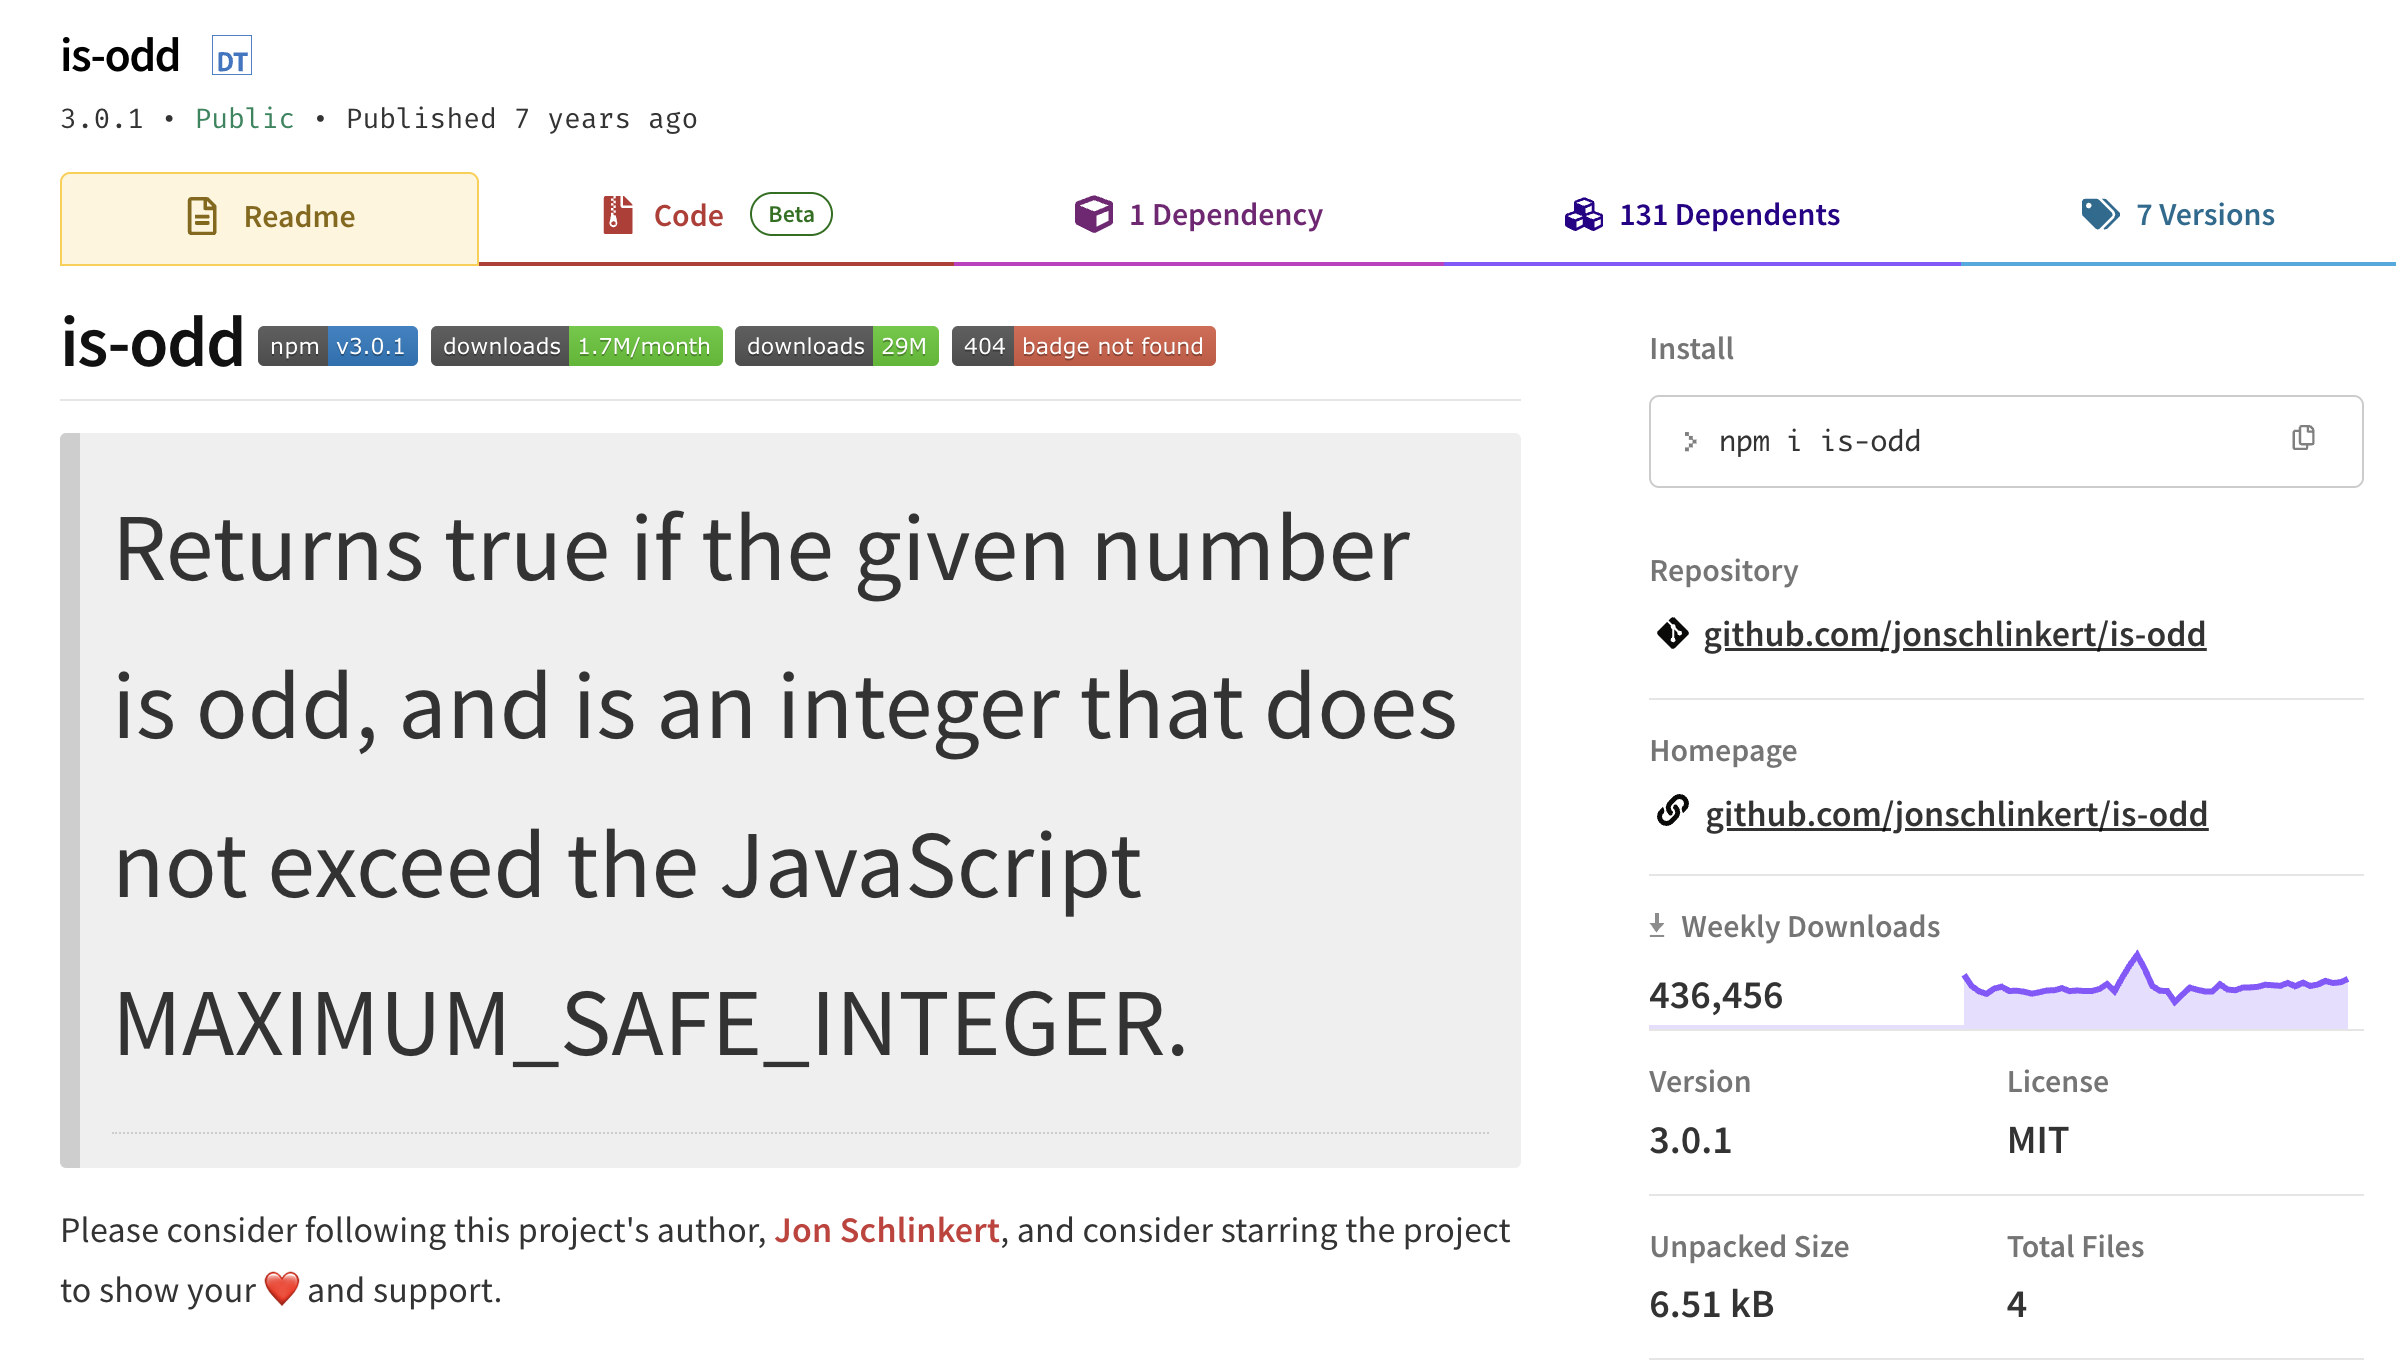
\includegraphics[width=0.7\linewidth,height=\textheight,keepaspectratio]{images/is-odd.png}

}

\caption{is-odd npm}

\end{figure}%

First define a function called \texttt{is\_even()} that takes an
\texttt{i32} (integer) and returns a \texttt{bool}.

\begin{Shaded}
\begin{Highlighting}[]
\KeywordTok{fn}\NormalTok{ is\_even(x}\OperatorTok{:} \DataTypeTok{i32}\NormalTok{) }\OperatorTok{{-}\textgreater{}} \DataTypeTok{bool} \OperatorTok{\{}
\NormalTok{    x }\OperatorTok{\%} \DecValTok{2} \OperatorTok{==} \DecValTok{0}
\OperatorTok{\}}
\end{Highlighting}
\end{Shaded}

We can use our already defined function inside of another:

\begin{Shaded}
\begin{Highlighting}[]
\KeywordTok{fn}\NormalTok{ is\_odd(x}\OperatorTok{:} \DataTypeTok{i32}\NormalTok{) }\OperatorTok{{-}\textgreater{}} \DataTypeTok{bool} \OperatorTok{\{}
    \OperatorTok{!}\NormalTok{is\_even(x)}
\OperatorTok{\}}
\end{Highlighting}
\end{Shaded}

\section{Exercise}\label{exercise-6}

Create a function called \texttt{mean()} that calculates the mean of a
\texttt{Vec\textless{}f64\textgreater{}}.

\begin{itemize}
\tightlist
\item
  In \texttt{main()}, create a vector \texttt{x} with 5 or more
  \texttt{f64} values.
\item
  Call \texttt{mean(x)} and print the result.
\end{itemize}

\begin{tcolorbox}[enhanced jigsaw, titlerule=0mm, coltitle=black, opacitybacktitle=0.6, bottomrule=.15mm, bottomtitle=1mm, colframe=quarto-callout-note-color-frame, toprule=.15mm, opacityback=0, rightrule=.15mm, leftrule=.75mm, breakable, left=2mm, colback=white, colbacktitle=quarto-callout-note-color!10!white, toptitle=1mm, title=\textcolor{quarto-callout-note-color}{\faInfo}\hspace{0.5em}{Note}, arc=.35mm]

Use \texttt{x.len()} to get the length and \texttt{as\ f64} to convert
it to a float.

\end{tcolorbox}

\subsection{Solution}\label{solution-6}

View solution

\begin{Shaded}
\begin{Highlighting}[]
\KeywordTok{fn}\NormalTok{ mean(x}\OperatorTok{:} \DataTypeTok{Vec}\OperatorTok{\textless{}}\DataTypeTok{f64}\OperatorTok{\textgreater{}}\NormalTok{) }\OperatorTok{{-}\textgreater{}} \DataTypeTok{f64} \OperatorTok{\{}
    \KeywordTok{let} \KeywordTok{mut}\NormalTok{ total }\OperatorTok{=} \DecValTok{0.0}\OperatorTok{;}
    \KeywordTok{let}\NormalTok{ n }\OperatorTok{=}\NormalTok{ x}\OperatorTok{.}\NormalTok{len()}\OperatorTok{;}
    \ControlFlowTok{for}\NormalTok{ xi }\KeywordTok{in}\NormalTok{ x }\OperatorTok{\{}
\NormalTok{        total }\OperatorTok{+=}\NormalTok{ xi}\OperatorTok{;}
    \OperatorTok{\}}
\NormalTok{    total }\OperatorTok{/}\NormalTok{ n }\KeywordTok{as} \DataTypeTok{f64}
\OperatorTok{\}}

\KeywordTok{fn}\NormalTok{ main() }\OperatorTok{\{}
    \KeywordTok{let}\NormalTok{ x }\OperatorTok{=} \PreprocessorTok{vec!}\NormalTok{[}\DecValTok{1.0}\OperatorTok{,} \DecValTok{2.0}\OperatorTok{,} \DecValTok{3.0}\OperatorTok{,} \DecValTok{4.0}\OperatorTok{,} \DecValTok{5.0}\NormalTok{]}\OperatorTok{;}
    \KeywordTok{let}\NormalTok{ result }\OperatorTok{=}\NormalTok{ mean(x)}\OperatorTok{;}
    \PreprocessorTok{println!}\NormalTok{(}\StringTok{"Mean is: \{\}"}\OperatorTok{,}\NormalTok{ result)}\OperatorTok{;}
\OperatorTok{\}}
\end{Highlighting}
\end{Shaded}

\chapter{Ownership}\label{ownership}

\begin{itemize}
\tightlist
\item
  last exercise we defined a function that takes
  \texttt{x:\ Vec\textless{}f64\textgreater{}}
\item
  this \emph{comsumes} the vector
\item
  If we try running this function \emph{twice} our code wont compile
\item
  This is because \texttt{x} was \emph{moved}.
\item
  In Rust a variable can be used only ONCE
\end{itemize}

\section{Borrowing}\label{borrowing}

\begin{itemize}
\tightlist
\item
  however it can be BORROWED many times
\item
  We want to borrow whenever we can
\item
  borrowing is recognized by the \texttt{\&} character in front of a
  variable
\item
  this means we can use its value by \emph{reference}
\item
  we cannot modify its value nor we can we move it.
\item
  only \emph{borrow} it.
\end{itemize}

\section{Exercise 1}\label{exercise-1-1}

rewrite \texttt{mean()} to use a \emph{reference} to `Vec

\subsection{Solution}\label{solution-7}

\begin{Shaded}
\begin{Highlighting}[]
\KeywordTok{fn}\NormalTok{ mean(x}\OperatorTok{:} \OperatorTok{\&}\DataTypeTok{Vec}\OperatorTok{\textless{}}\DataTypeTok{f64}\OperatorTok{\textgreater{}}\NormalTok{) }\OperatorTok{{-}\textgreater{}} \DataTypeTok{f64} \OperatorTok{\{}
    \KeywordTok{let} \KeywordTok{mut}\NormalTok{ total }\OperatorTok{=} \DecValTok{0.0}\OperatorTok{;}
    \KeywordTok{let}\NormalTok{ n }\OperatorTok{=}\NormalTok{ x}\OperatorTok{.}\NormalTok{len()}\OperatorTok{;}

    \ControlFlowTok{for}\NormalTok{ xi }\KeywordTok{in}\NormalTok{ x }\OperatorTok{\{}
\NormalTok{        total }\OperatorTok{+=}\NormalTok{ xi}\OperatorTok{;}
    \OperatorTok{\}}
\NormalTok{    total }\OperatorTok{/}\NormalTok{ n }\KeywordTok{as} \DataTypeTok{f64}
\OperatorTok{\}}
\end{Highlighting}
\end{Shaded}

\section{Slices}\label{slices}

\begin{itemize}
\tightlist
\item
  a contiguous block of the same type
\item
  available only as references
\item
  we always know the length of a slice i.e.~\texttt{.len()} is available
\item
  denoted as \texttt{\&{[}T{]}} (again remember \texttt{T} is a generic
  type)---e.g.~\texttt{\&{[}f64{]}} or \texttt{\&{[}i32{]}}
\item
  in general, if we can use a slice we should
\item
  if we cannot use a slice, use a reference
\item
  if we cannot use a reference move it
\end{itemize}

\section{Exercise}\label{exercise-7}

\begin{itemize}
\tightlist
\item
  Rewrite \texttt{mean()} to use a slice of f64
\end{itemize}

\subsection{Solution}\label{solution-8}

\begin{Shaded}
\begin{Highlighting}[]
\KeywordTok{fn}\NormalTok{ mean(x}\OperatorTok{:} \OperatorTok{\&}\NormalTok{[}\DataTypeTok{f64}\NormalTok{]) }\OperatorTok{{-}\textgreater{}} \DataTypeTok{f64} \OperatorTok{\{}
    \KeywordTok{let} \KeywordTok{mut}\NormalTok{ total }\OperatorTok{=} \DecValTok{0.0}\OperatorTok{;}
    \KeywordTok{let}\NormalTok{ n }\OperatorTok{=}\NormalTok{ x}\OperatorTok{.}\NormalTok{len()}\OperatorTok{;}

    \ControlFlowTok{for}\NormalTok{ xi }\KeywordTok{in}\NormalTok{ x }\OperatorTok{\{}
\NormalTok{        total }\OperatorTok{+=}\NormalTok{ xi}\OperatorTok{;}
    \OperatorTok{\}}
\NormalTok{    total }\OperatorTok{/}\NormalTok{ n }\KeywordTok{as} \DataTypeTok{f64}
\OperatorTok{\}}
\end{Highlighting}
\end{Shaded}

\chapter{Iterators}\label{iterators}

\begin{itemize}
\item
  The goal of this section is to go over iterators.
\item
  \texttt{.iter()} does not \emph{move} (consume) the item
  \texttt{.into\_iter()} does
\item
  each element of \texttt{.iter()} is a reference whereas
  \texttt{.into\_iter()} gives you the value itself
\item
  a for loop uses \texttt{.into\_iter()} (consuming)
\item
  First cover \texttt{.into\_iter()} to create a consuming iterator this
  way the inner type is not a reference
\item
  We can talk about the basic methods for iterators:

  \begin{itemize}
  \tightlist
  \item
    \texttt{.sum()}
  \item
    \texttt{.min()}
  \item
    \texttt{.max()}
  \item
    \texttt{.min()}: not floating point arith issues here
  \item
    \texttt{.max()}: note floating point arith issues here
  \item
    \texttt{.enumerate()}
  \end{itemize}
\item
  then the next section we can
\end{itemize}

\section{Exercises}\label{exercises}

\begin{itemize}
\tightlist
\item
  calculate the mean using an iterator
\item
  use an enumerated for loop to sum only even numbers
\item
  calculate the standard deviation
\end{itemize}

\chapter{Defining Struct(ure)s}\label{defining-structures}

\begin{itemize}
\tightlist
\item
  PascalCase naming convention
\item
  deriving traits:

  \begin{itemize}
  \tightlist
  \item
    debug, clone
  \end{itemize}
\item
  destructuring assignment
\end{itemize}

\section{Exercise}\label{exercise-8}

\begin{itemize}
\tightlist
\item
  Define a struct called \texttt{Point} which has two fields \texttt{x},
  and \texttt{y}
\item
  Create a new \texttt{Point} struct
\item
  Destructure the point
\end{itemize}

\chapter{Enum(eration)s}\label{enumerations}

\section{Exercise}\label{exercise-9}

\begin{itemize}
\tightlist
\item
  Create an enum called \texttt{Measure}
\item
  Create a new method \texttt{distance()} for our point struct
\end{itemize}

\begin{Shaded}
\begin{Highlighting}[]
\KeywordTok{enum}\NormalTok{ Measure }\OperatorTok{\{}
\NormalTok{    Euclidean}\OperatorTok{,}
\NormalTok{    Haversine}\OperatorTok{,}
\OperatorTok{\}}

\KeywordTok{impl}\NormalTok{ Point }\OperatorTok{\{}
    \KeywordTok{fn}\NormalTok{ haversine\_distance(}\OperatorTok{\&}\KeywordTok{self}\OperatorTok{,}\NormalTok{ destination}\OperatorTok{:} \OperatorTok{\&}\DataTypeTok{Self}\NormalTok{) }\OperatorTok{{-}\textgreater{}} \DataTypeTok{f64} \OperatorTok{\{}
        \KeywordTok{let}\NormalTok{ radius }\OperatorTok{=} \DecValTok{6\_371\_008.7714}\OperatorTok{;}
        \KeywordTok{let}\NormalTok{ theta1 }\OperatorTok{=} \KeywordTok{self}\OperatorTok{.}\NormalTok{y}\OperatorTok{.}\NormalTok{to\_radians()}\OperatorTok{;}
        \KeywordTok{let}\NormalTok{ theta2 }\OperatorTok{=}\NormalTok{ destination}\OperatorTok{.}\NormalTok{y}\OperatorTok{.}\NormalTok{to\_radians()}\OperatorTok{;}
        \KeywordTok{let}\NormalTok{ delta\_theta }\OperatorTok{=}\NormalTok{ (destination}\OperatorTok{.}\NormalTok{y }\OperatorTok{{-}} \KeywordTok{self}\OperatorTok{.}\NormalTok{y)}\OperatorTok{.}\NormalTok{to\_radians()}\OperatorTok{;}
        \KeywordTok{let}\NormalTok{ delta\_lambda }\OperatorTok{=}\NormalTok{ (destination}\OperatorTok{.}\NormalTok{x }\OperatorTok{{-}} \KeywordTok{self}\OperatorTok{.}\NormalTok{x)}\OperatorTok{.}\NormalTok{to\_radians()}\OperatorTok{;}
        \KeywordTok{let}\NormalTok{ a }\OperatorTok{=}\NormalTok{ (delta\_theta }\OperatorTok{/} \DecValTok{2f64}\NormalTok{)}\OperatorTok{.}\NormalTok{sin()}\OperatorTok{.}\NormalTok{powi(}\DecValTok{2}\NormalTok{)}
            \OperatorTok{+}\NormalTok{ theta1}\OperatorTok{.}\NormalTok{cos() }\OperatorTok{*}\NormalTok{ theta2}\OperatorTok{.}\NormalTok{cos() }\OperatorTok{*}\NormalTok{ (delta\_lambda }\OperatorTok{/} \DecValTok{2f64}\NormalTok{)}\OperatorTok{.}\NormalTok{sin()}\OperatorTok{.}\NormalTok{powi(}\DecValTok{2}\NormalTok{)}\OperatorTok{;}
        \DecValTok{2f64} \OperatorTok{*}\NormalTok{ a}\OperatorTok{.}\NormalTok{sqrt()}\OperatorTok{.}\NormalTok{asin() }\OperatorTok{*}\NormalTok{ radius}
    \OperatorTok{\}}
\OperatorTok{\}}
\end{Highlighting}
\end{Shaded}

\part{Building Rust based R Packages}

\chapter{Building Rust based R
Packages}\label{building-rust-based-r-packages-1}




\end{document}
